\section{Experimental Setup}	\label{sec:related_works}

It was decided to develop and test MABDI in a completely simulated environment
so that all results could be repeatable and also to facilitate the ability to
debug during the development process. This ability was truly invaluable as some
components of the algorithm proved to be complex from an implementation
perspective. Examples include the code to project points from the depth image to
real-world coordinates and the code for the surface reconstruction method. Being
able to debug the system by stopping the simulation at any point and inspecting
objects was nearly a necessity. In addition, we can now compare the resultant
global mesh to ground truth.

\subsection{Simulation Parameters}

The simulation was designed to be highly configurable and is implemented by a
class named MabdiSimulate. The class is initialized with parameters that control
all aspects of the simulation. Parameters of a particular importance are
discussed in more detail here:

\begin{itemize}
    \item  Environment - This parameter specifies the environment used to generate
    the simulated depth images. \textit{Table} is an environment consisting of a
    table and two cups placed on the table. The table is 1 meter tall.
    \textit{Bunnies} is an environment consisting of three bunnies who are
    around 1.5 meters tall. These bunnies are created using the Stanford Bunny
    \cite{Turk1994}, a well known data set in computer graphics.
    \item Noise - If true, adds noise to the depth image of the simulated sensor.
    \item Dynamic - If true, adds an object during the simulation. In the case
    of this analysis, a third bunny is added half-way through the simulation.
\end{itemize}

% parameters chosen the experimental runs
For this paper we will be exploring three experimental runs to demonstrate the
ability of the MABDI implementation to generate valid results. Additionally, the
experimental runs will be able to show the capabilities of the MABDI algorithm
such as handling object addition in the environment.

\begin{table}[h]
  \caption{Description of the experimental runs.}
  \label{tab:run}
  \begin{footnotesize}
  \begin{center}
    \begin{tabular}{|l|c|c|c|}
    \hline
           & Environment & Noise   & Dynamic \\\hline
    Run 1	 & Table       & False   & False       \\
    Run 2  & Bunnies     & True    & False       \\
    Run 3  & Bunnies     & True    & True       \\
    \hline
    \end{tabular}
  \end{center}
  \end{footnotesize}
\end{table}

All experimental runs define a helical path for the sensor to follow during the
simulation. The path circles the objects in the environment twice. A helical
path was chosen because it returns to a part of the environment that has been
already mapped and is thus ``known'' to the global mesh. Also, because the path
is a helix and not just a circle, the sensor views the environment from a
slightly different position on each pass.

\subsection{Analysis of Simulated Noise}

In order to realistically simulate the sensor in a real-world environment we add noise to the depth image $D$. See Fig. \ref{fig:system}. The 

As new RGB-D sensors have been developed such, as the Asus Xtion and the Kinect for Xbox One, the accuracy of the sensors has improved \cite{lachat2015first}.

Popularly accepted noise model for the kinect sensor. \cite{Khoshelham2012}

% Can add equation showing addition of noise if there is space later

% Viewpoint coordinates to real-world coordinates analysis. Viewpoint coordinates
% are obtained when a mesh is rendered into a render window, and can be
% transformed to real-world coordinates using the transformation matrix of the
% camera. Noise is added in simulation to the viewpoint coordinates. This graph
% shows the effect of that noise in real-world coordinates.

\begin{figure}[h]%[thpb]
\centering
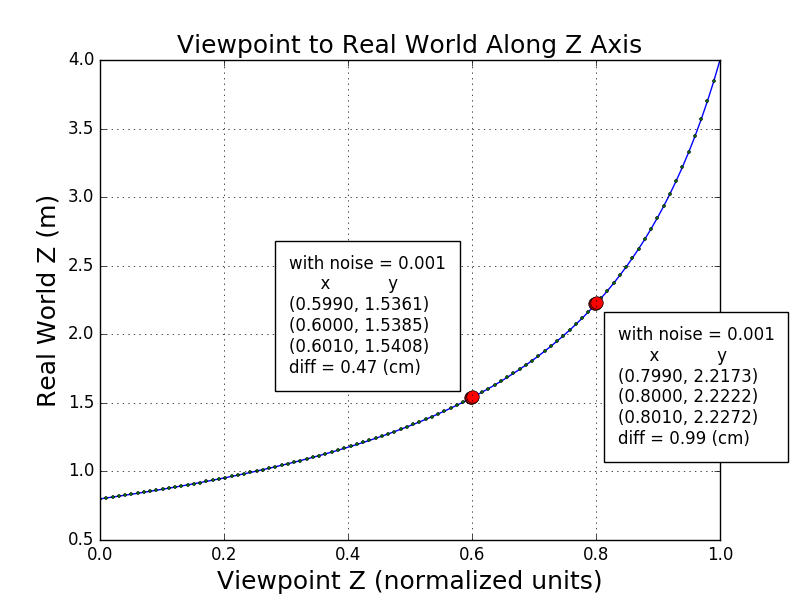
\includegraphics[width=.5\textwidth]{figures/plot_depth.png}
\caption{Viewpoint coordinates to real world coordinates analysis.}
\label{fig:depth}
\end{figure}
